## Recursividad {.fragile}

\bgncolumns

\column{0.6\textwidth}

\vspace{-1em}

\bgnblockgood[wd=.8\textwidth,centered]
Maurits Cornelis Escher
\trmblockgood

\centering ``Drawing hands''

\column{0.4\textwidth}
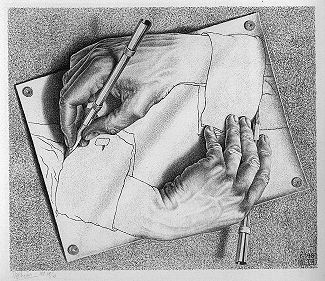
\includegraphics[width=0.8\textwidth,valign=t]{img/DrawingHands.jpg}
\trmcolumns

- Artista holandés.
- Célebre por sus obras inspiradas en temas relacionados con la matemática.
- Jugó impecablemente con figuras imposibles, desafiando las dimensiones espaciales.

- La paradoja en esta obra: ¿cuál es la mano que comenzó el dibujo?

## Recursividad {.fragile}

\simpleTitle{La base de la recursividad está en la naturaleza:}

¿Qué es un árbol?

- Un árbol es una rama.
- De una rama salen varias ramas.
- De una rama salen varias ramas.
- De una rama salen varias ramas.
- De una rama salen varias ramas.
...
- De una rama sale una hoja o una flor.

\bgnblocknormal
¿En qué se asemeja esto a un río?
\trmblocknormal

## Recursividad {.fragile}

\simpleTitle{Definamos entonces recursividad:}

\pause

\bgnblockdefinition
Para entender la \structure{recursividad},

\pause

primero hay que entender la \structure{recursividad}.

\trmblockdefinition

\bgncolumns

\column{.7\textwidth}

\only{<5>}{%

\footnotesize
\begin{itemize}
\item Para resolver su duda llame al 12345.
\item Usted ha llamado al 12345. Para contestar sus dudas, corte y marque el 12345.
\item Usted ha llamado al 12345. Para contestar sus dudas, corte y marque el 12345.
\item Usted ha llamado al 12345. Para contestar sus dudas, corte y marque el 12345.
\end{itemize}

}

\column{.3\textwidth}

\only{<4->}{%

\includegraphics[width=\textwidth,valign=t]{img/manthinking-1f914.pdf}
}

\trmcolumns

## Recursividad {.fragile}

\simpleTitle{Veamos una definición más amable:}

\bgnblockdefinition
\flushleft \vspace{-2ex} Un proceso es \structure{recursivo} si:
\vspace{1ex}

1. Tiene un caso base.
1. Hay una regla principal que se llama a sí misma
    - \normalsize \vspace{.4ex} Pero en cada llamado se va reduciendo.
    - Hasta finalmente llegar al caso base.

\vspace{.5ex}
\trmblockdefinition

\vfill

\bgncolumns
\column{.33\textwidth}
\centering

\includegraphics[width=.6\textwidth,valign=t]{img/spiral.png}
\column{.33\textwidth}
\centering

\includegraphics[width=.6\textwidth,valign=t]{img/samsung-shell.png}
\column{.33\textwidth}
\centering

\includegraphics[width=.6\textwidth,valign=t]{img/coffee_v10_2615.pdf}
\trmcolumns

## Recursividad {.fragile}

\simpleTitle{Ejemplos}

- Elevar a potencias

$$ 2^0 = 1 $$
$$ 2^n = 2 * 2^{n-1} $$

- Factorial

$$ 0! = 1 $$
$$ n! = n * (n-1)! $$

